%\documentclass[referee]{aa} % for a referee version
%\documentclass[onecolumn]{aa} % for a paper on 1 column  
%\documentclass[longauth]{aa} % for the long lists of affiliations 
%\documentclass[letter]{aa} % for the letters 
\documentclass{aa}


\usepackage{txfonts}
\usepackage{natbib}

\usepackage{graphicx}
\usepackage{subcaption}

\usepackage{color}
\usepackage{hyperref}
\hypersetup{colorlinks=true,allcolors=[rgb]{0,0,0.8}}

\usepackage{xcolor,soul}
\sethlcolor{yellow}

% the three lines suppress the hyperref 'link empty' warnings
% explanation at: https://tex.stackexchange.com/questions/345764/journal-class-shows-package-hyperref-warning-suppressing-link-with-empty-targe
\makeatletter
\renewcommand*\aa@pageof{, page \thepage{} of \pageref*{LastPage}}
\makeatother

% text highlighting
\usepackage{soul}
\sethlcolor{yellow}

\usepackage{showyourwork}

\begin{document} 
\authorrunning{Kenworthy et al.}
\titlerunning{ERIS gvAPP}
  \title{The ERIS gvAPP Coronagraph: theoretical and on-sky performance}

   \author{M. A. Kenworthy
          \inst{1}
          \and
          F. Dannert
          \inst{2}
          \and
          J. Hayoz
          TBD
          \inst{2}
          \and
          D. Doelman
          \inst{1}
          \and
          Ben Sutlieff
          \inst{3}
          \and
          F. Snik
          \inst{1}
        \and
        S. Quanz
        \inst{2}
          }

   \institute{Leiden Observatory, University of Leiden,
   PO Box 9513, 2300 RA Leiden, The Netherlands\\
   \email{kenworthy@strw.leidenuniv.nl} \\
   \and 
      ETH Zurich, Switzerland
      \and
      Edinburgh
}
   \date{Received \today; accepted XXXX}

% \abstract{}{}{}{}{} 
% 5 {} token are mandatory
 
  \abstract
  % context heading (optional)
  % {} leave it empty if necessary  
   {}
  % aims heading (mandatory)
   {We describe the gvAPP coroangraph for ERIS.}
  % methods heading (mandatory)
   {On sky observations from the commissioning run enabled characterisation of the gvAPP performance.}
  % results heading (mandatory)
   {Excellent matching with the prescribed pattern.
   %
   Different wavelength performance.}
  % conclusions heading (optional), leave it empty if necessary 
   {}

   \keywords{instrumentation -- coronagraphs}

   \maketitle
%
%-------------------------------------------------------------------

   \section{Introduction}

%\begin{figure}
%%    \begin{centering}
 %   \includegraphics[width=0.5\textwidth]{figures/gvapp_psf.pdf}
 %   \caption{gvAPP psf as seen in ERIS.
%              }
%    \label{fig:erisapp}
%    \script{plot_eris_gvapp_psf.py}
%    \end{centering}
%\end{figure}
The Enhanced Resolution Imager and Spectrograph for the VLT \citep[ERIS; ][]{2023A&A...674A.207D} is an diffraction limited 1.5 to 5 micron imager and spectrograph, providing a 20 arcsecond field of view and $R=5000$ spectroscopy using an integral field unit.
%
It is composed of two parts, the integral field spectrograph SPIFFIER (REF) and the diffraction-limited high angular resolution imager NIX (REF).



\section{Phase pattern design}

\hl{MAK, DD}

\begin{itemize}
    \item The ERIS gvAPP designed in 2018
    
    \item The design steps follow \cite{2021ApOpt..60D..52D}
    \item The design takes advantage of the small spiders and relatively small central obscuration with an aggressive design contrast at a small IWA.
    \item The vAPP is also a cold stop.  To account for pupil wander and drifts, the pupil was undersized.  
    \item The dark zones are broadened in the grating direction to account for wavelength smearing.
    \item The direction of the grating and dark zones was chosen to  minimize the impact of spider diffraction in the dark zone, which would reduce the design Strehl ratio.
    \item The grating has 25 cycles over the diameter, resulting in a 25 $\lambda/D$ separation between the coronagraphic PSF and the leakage term. This separation was chosen to minimize the impact of the leakage PSF intensity and account for the width of the dark zones.
    \item Lower-intensity reference PSFs the same separation but rotated  90 degrees have been added as an astrometric and photometric reference.
    \item  The coronagraphic PSFs have additional dark zones underneath the leakage term and reference PSFs to reduce the impact of residual aberrations on their photometry.

\end{itemize}


\begin{figure}
    \centering
    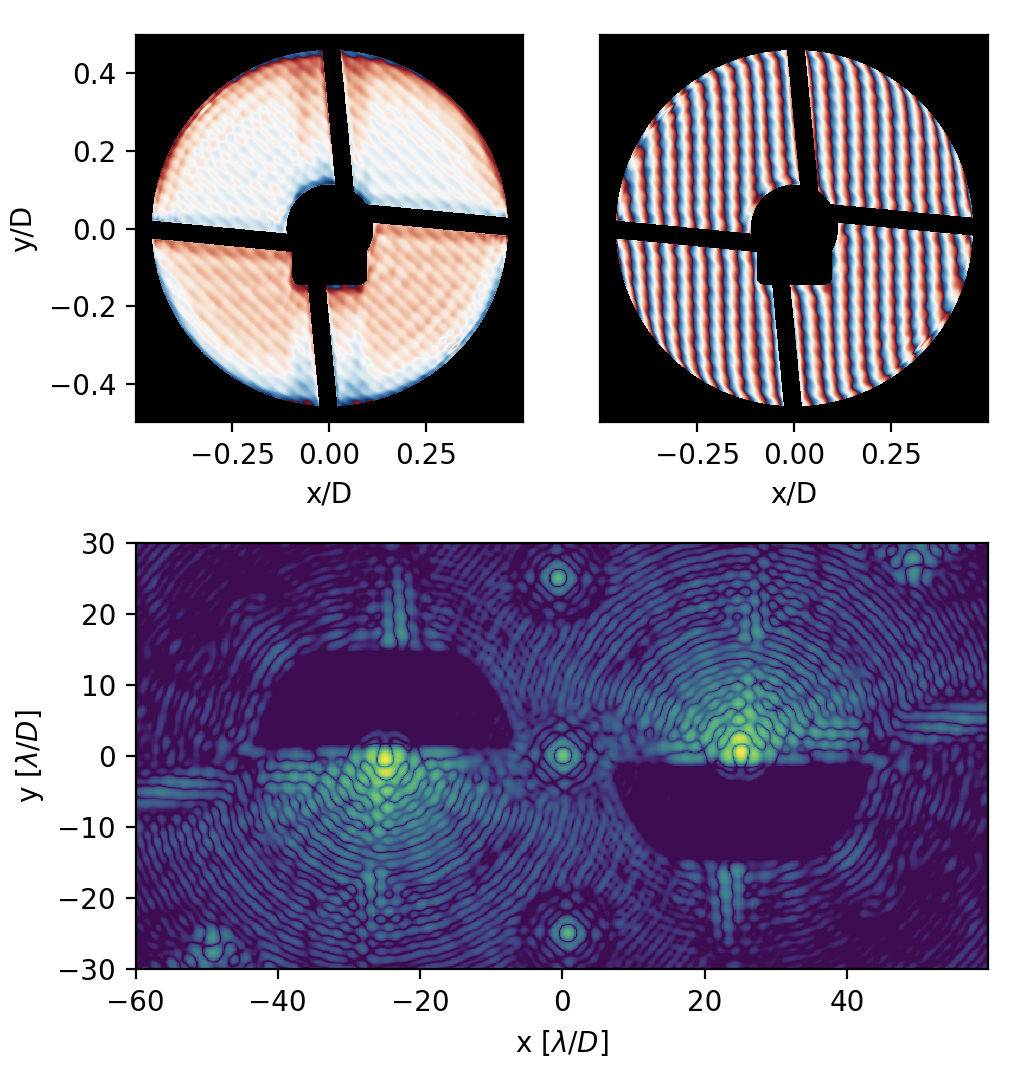
\includegraphics[width=0.45\textwidth]{figures/ERIS_phase_place_holder.png}
    \caption{The ERIS gvAPP phase pattern design and and simulated PSF.}
    \label{fig:gvAPP_phase}
\end{figure}

\begin{table}[h!]
\label{tab:design_param}
\caption{Design parameter values of the ERIS gvAPP}
\begin{tabular}{c|c|c|c|c|c}
     Design & IWA & IWA & OWA & OWA  & Strehl\\
     parameter&& contrast&& contrast&\\
     \hline     
     &$[\lambda/D]$& &$[\lambda/D]$ & & [\%]\\
    \hline
     Value & 2.2 &  $10^{-4}$ &15 &  $10^{-5}$ & 50.9\\
\end{tabular}
\end{table}

\section{Optical construction of the gvAPP}

\hl{MAK, DD}
\begin{itemize}
    \item Component manufactured by ImagineOptix in 2018
    \item Two components manufactured, spare has slightly worse quality.
\end{itemize}

\textbf{Optical layering, flatness, wedge}
\begin{itemize}
    \item The optics stack of the gvAPP consists of four individual substrates glued together.
    \item The number of substrates needed to be four due to manufacturing limitations and instrument constraints.
    \begin{itemize}
        \item The AR-coating could not be applied to the opposite side of the aluminium mask.
        \item The liquid-crystal film could not be applied on the wedged substrate.
    \end{itemize}
    \item Amplitude mask is Aluminum thickness about 300 nm, OD $>$ 4.
    \item The wedge is pointing North South, orthogonal to the grating
    \item The stack thickness is 7.55/7.39 mm (top, bottom), as measured with calipers. Resulting wedge angle is 0.44 degrees.
    \item The overall diameter is 20.95 mm.
    \item Centricity of clear aperture: Part A: 0.020 mm from center of 21 mm substrates
    \item Anti-reflection coatings are each $< 0.5$ \% average reflectance, verified by vendor
    \item Glue is NOA-61, aged 10-hrs at 50°C.
\end{itemize}



\begin{figure}
    \centering
    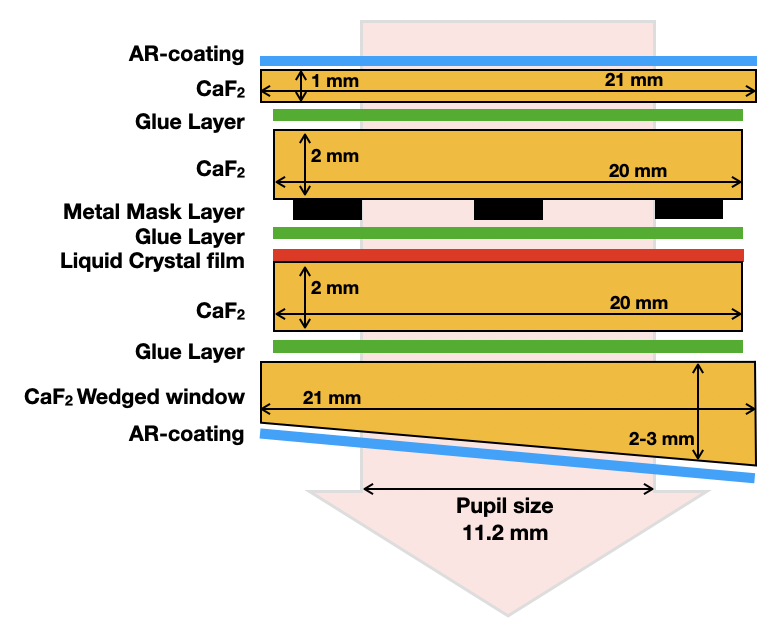
\includegraphics[width=0.45\textwidth]{figures/gvAPP_stack.png}
    \caption{The ERIS gvAPP optical layering.}
    \label{fig:optical_layering}
\end{figure}

\begin{figure}
\centering
\begin{subfigure}{.25\textwidth}
  \centering
    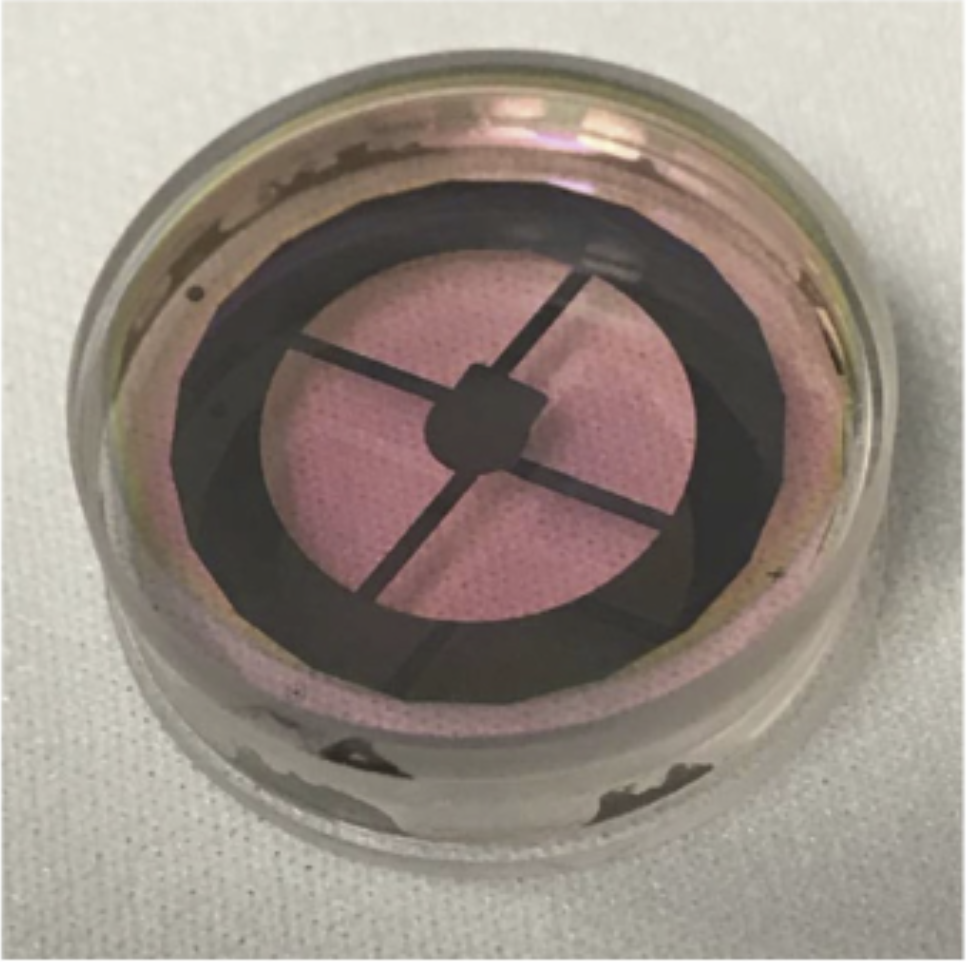
\includegraphics[width=0.9\textwidth]{figures/ERIS_gvAPP_image.png}
\end{subfigure}%
\begin{subfigure}{.25\textwidth}
  \centering
    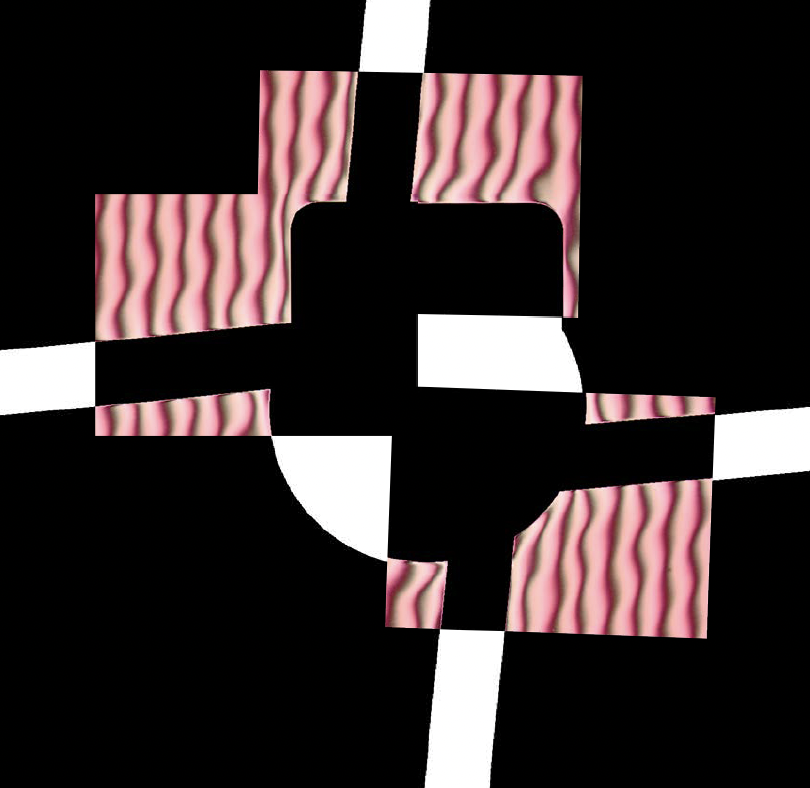
\includegraphics[width=0.915\textwidth]{figures/microscope_image.png}
  \label{fig:microscope_image}
  \label{fig:sub2}
\end{subfigure}
    \caption{Left: Image of the manufactured ERIS gvAPP. Right: Three stitched microscope images of the ERIS gvAPP between crossed polarizers. Images from ImagineOptix. }
\label{fig:test}
\end{figure}

\textbf{Transmission curve}
\begin{itemize}
    \item Both the glue and liquid crystal layers display absorption features in the thermal infrared and result in an average 2-5 $\mu$m transmission of 61.3\%. 
    \item The transmission was measured in the clear aperture and includes all substrates, glue layers, LCP layer, and anti-reflection coatings.
    \item A comparable transmission curve of the LBT dgvAPP can be found in \cite{2022AJ....163..217D}. 
    \item The overall transmission in is $\sim 90\%$ in K-band, $\sim 50\%$ in L-band, $\sim 40\%$ in M-band. 
    \item The absorption feature at $3.3 \mu$m goes to 0\% transmission, rendering L-short observations ineffective. This absorption feature is caused by absorption in both the glue and liquid-crystal layers.
    \item The significant absorption in L-band and M-band will impact the gvAPP performance by increasing the photon noise of the thermal background.
\end{itemize}

\begin{figure}
    \centering
    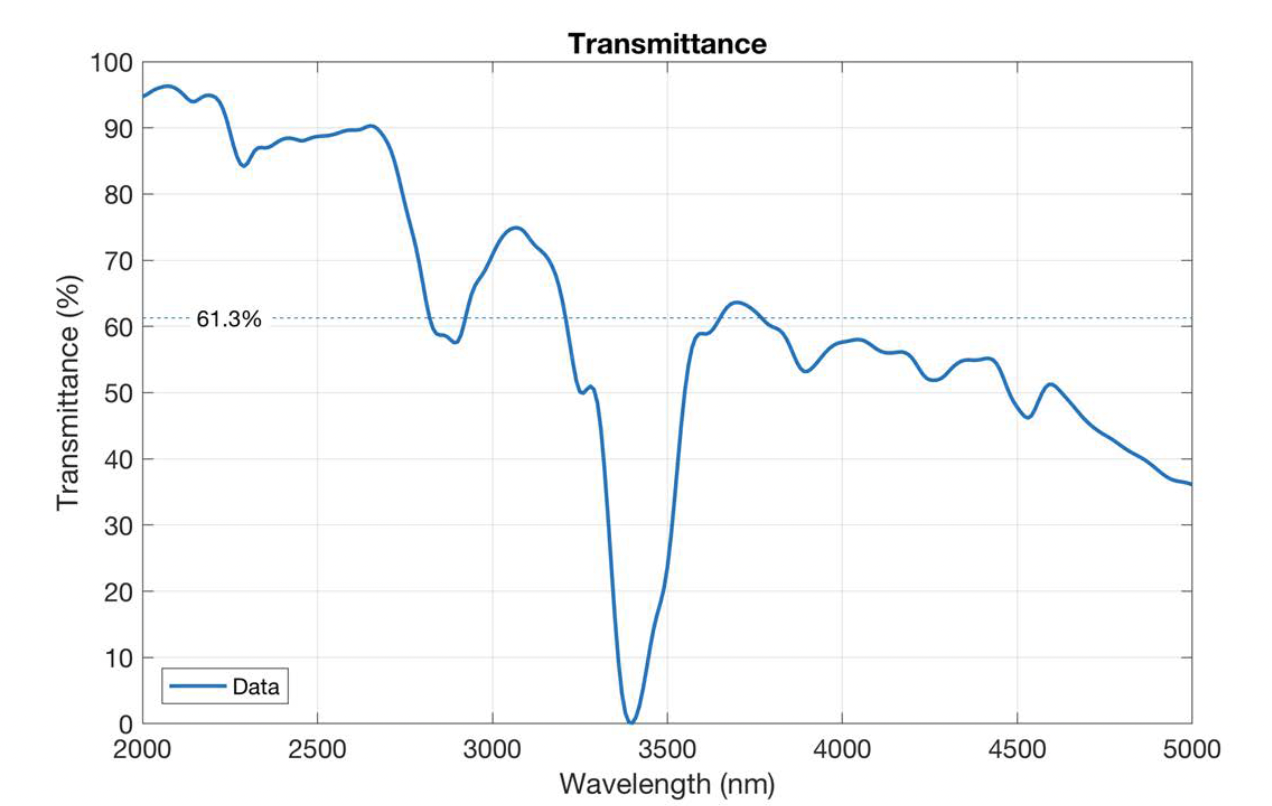
\includegraphics[width=0.45\textwidth]{figures/Transmission_gvAPP.png}
    \caption{Transmission of the gvAPP as a function of wavelength. }
    \label{fig:optical_layering}
\end{figure}

\section{Summary cryogenic tests}

\hl{MAK, DD}

\begin{itemize}
    \item gvAPP was tested at ETH Zurich cryogenic testbed \citep{2018SPIE10702E..3YB,2021JATIS...7d5001B}. 
    \item The testbed was operated using a narrowband filter centered at 2.006 $\mu$m with a full width at half maximum of 0.045 $\mu$m.  
    \item The first cryogenic tests confirmed  that the morphology, overall throughput, and core intensity of the gvAPP PSF compared with a nominal VLT PSF is consistent with the theoretical predictions.
    \item After upgrades of the cryogenic testbed, it was discovered that the measured gvAPP PSF had a reduced dark zone contrast compared to the theoretical PSF. In the paper the authors find that the dark zone contrast was limited by the testbed itself instead of the gvAPP optical quality. The reduction in contrast can be explained by optical surface polishing errors with a power-law power spectral density, combine with some defocus and jitter.
\end{itemize}

Anne Boehle discussion from her paper

XXX TAKEN from ANNA's PAPER! This is David's original image...

Look at this photograph... Figure~\ref{fig:sim_results}.

Glue throughput curve

Total throughput curve

\begin{figure*}
    \centering
    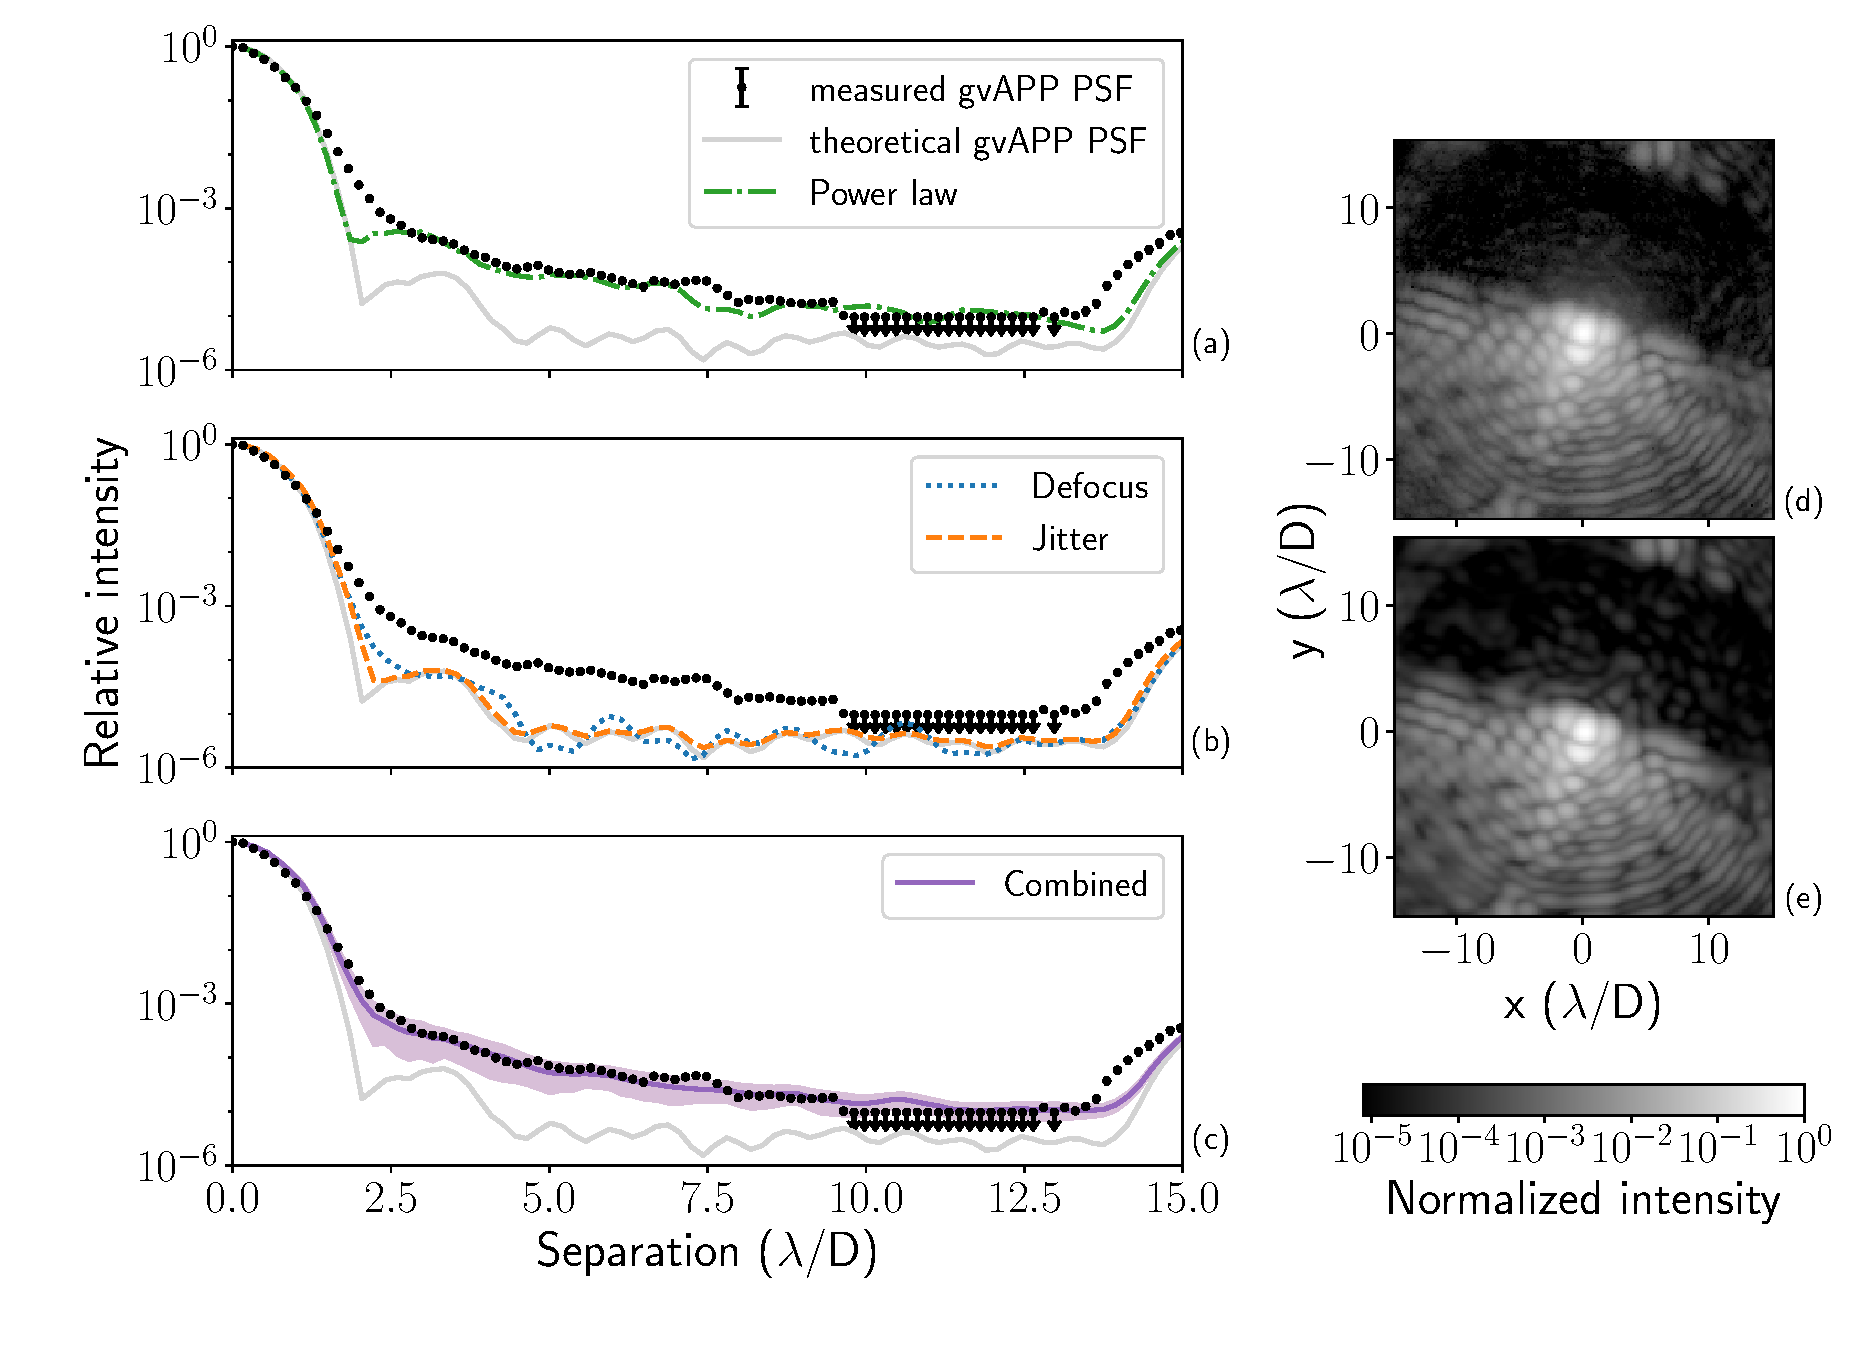
\includegraphics[width=0.95\textwidth]{figures/contrast_curve_withpsfs.pdf}
    \caption{Results from the simulations of the aberrations  observed in the gvAPP PSF.
    %
    The left column displays the simulated contrast curves when applying a a single realization of a power law aberration to simulate polishing errors (panel a), defocus and jitter aberrations (panel b), and all 3 aberrations combined including the average of 100 power law realizations and the 1$\sigma$ spread (panel c).
    %
    Each simulated contrast curve is compared to the data (black points) and to the theoretical gvAPP PSF (gray line).
    %
    The right column shows the test bench data of the left gvAPP PSF (panel d) compared to the simulated PSF with all 3 aberrations included (panel e).
    %
    We find that including polishing errors adds flux to the gvAPP dark hole as seen in the test bench measurements and that adding defocus and jitter smooths the PSF and makes the inner and outer edges of the dark hole line up with the measurements.
    %
    The combination of all three aberrations can explain the data very well in terms of the contrast curve and the PSF morphology.}
    \label{fig:sim_results}
\end{figure*}




\section{On-sky PSF comparison with model PSF}


\subsection{narrow band PSF on-sky}

\subsection{Current measured on-sky}

\begin{figure*}
    \centering
    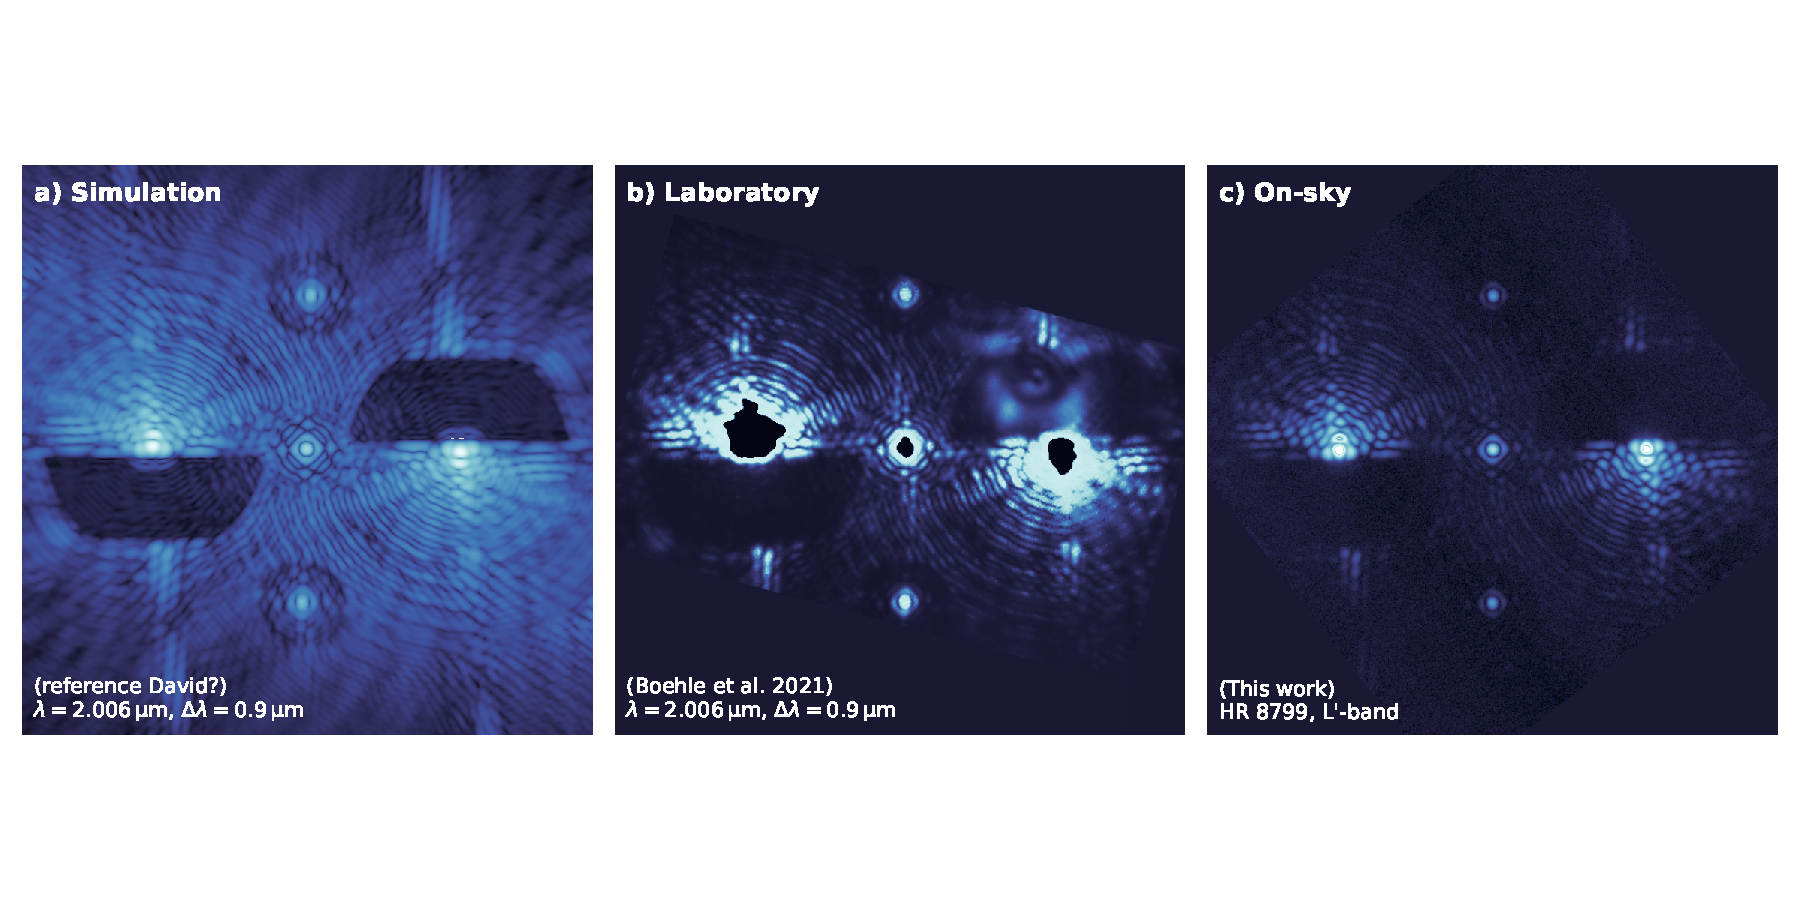
\includegraphics[width=0.95\textwidth]{figures/app_psf_model_lab_sky.pdf}
    \caption{Todo.}
    \label{fig:app_psf_comp}
\end{figure*}

\begin{figure}
    \centering
    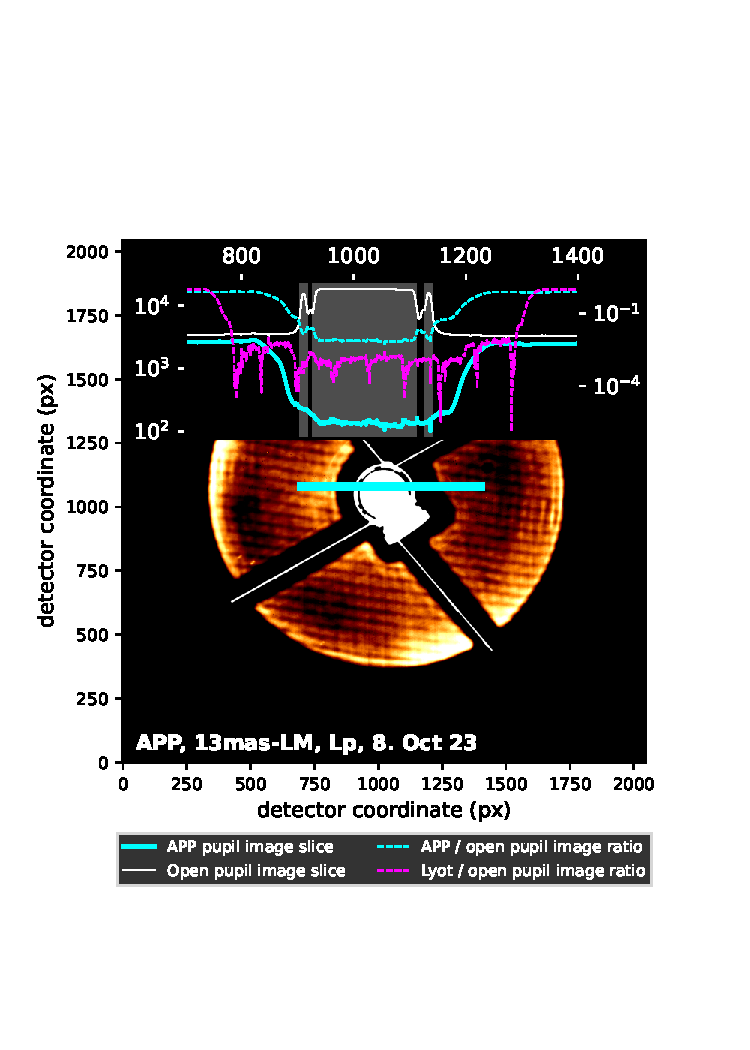
\includegraphics[width=0.45\textwidth]{figures/pupil_image_lp.pdf}
    \caption{Todo.}
    \label{fig:lprime_cc}
\end{figure}

\hl{JH, FD}

\subsection{IB on sky}

JH, FD

DD to meet with Ben Sutlieff Friday 14:00

left/right PSF brightness is not the same. hints at circular instrumentation systematics in ERIS???

Structure in the telescope pupil shows striping similar to the grating for the gvAPP - DD confirmed in 15/08/2024 email that these fringes are in the pattern (they create the reference holograms), and so a bit of Fresnel propagation will likely give the intensity variations.

Should look into why the spiders are so much thicker and what the bright ring is. Suspect this not only Fresnel propagation.

\subsection{Wavelength performance predicted and measured}
\hl{JH, FD, MAK}

\section{Contrast curves}

\subsection{Current measured on-sky}
\begin{figure}
    \centering
    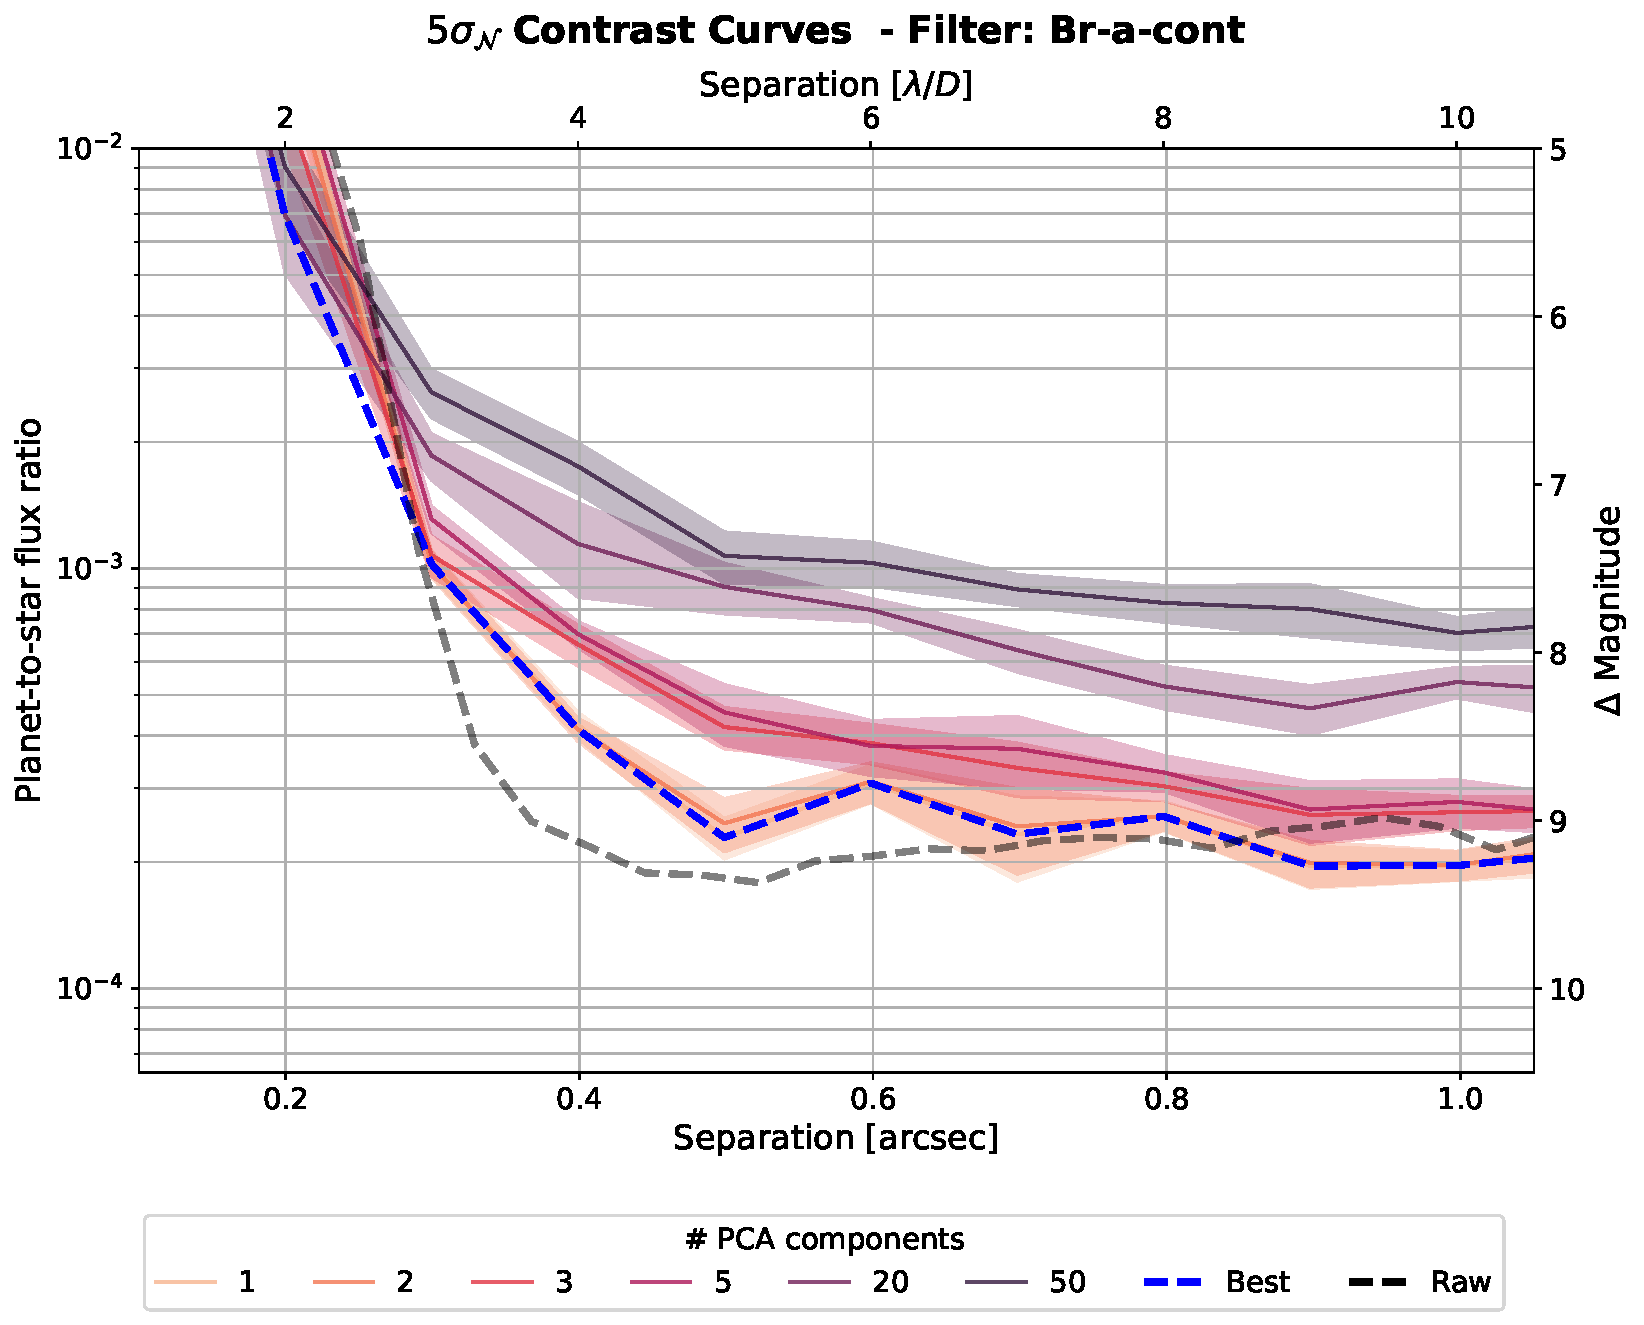
\includegraphics[width=0.45\textwidth]{figures/Contrast_curve_HR8799_Br-cont.pdf}
    \caption{Todo.}
    \label{fig:lprime_cc}
\end{figure}

\hl{JH, FD, DD, BS}

Include K-peak data from B.S.

\subsection{Predicted performance for broad bands}
\hl{JH, FD, DD}
Idea: take the contrast curve in K-peak (from BS), extrapolate it to the Kband (using the higher bandpass, and ignoring the changing sky background).

%------------------------
\section{Conclusions}\label{sec:conclusion}


\begin{itemize}
    \item gvAPP works to the design described, beamswitches perfectly, very easy to use.
    \item gvAPP successfully pushes diffraction halo below the wind driven halo from the atmosphere and AO system performance.
    \item L band limited by large sky background from warm optics in ERIS optical path and poor transmission due to multiple glue layers in ERIS gvAPP.
    \item Detector pattern noise and artifacts limit the K band reduction
    \item Future ELT instruments will minimise glue layers and increase strehl ratio for the same PSF contrast to improve planet throughput.
\end{itemize}

\subsection{Impact on future designs for ELT class telescopes}

Ask Olivier and Gilles

\hl{Everyone!}

Minimise the number of glue layers (2 is probably minimum)



\begin{acknowledgements}

ADD YOUR ACKNOWLEDGEMENTS HERE

This research has used the SIMBAD database, operated at CDS, Strasbourg, France \citep{wenger2000}.
%
This work has used data from the European Space Agency (ESA) mission {\it Gaia} (\url{https://www.cosmos.esa.int/gaia}), processed by the {\it Gaia} Data Processing and Analysis Consortium (DPAC, \url{https://www.cosmos.esa.int/web/gaia/dpac/consortium}).
%
Funding for the DPAC has been provided by national institutions, in particular the institutions participating in the {\it Gaia} Multilateral Agreement.
%
To achieve the scientific results presented in this article we made use of the \emph{Python} programming language\footnote{Python Software Foundation, \url{https://www.python.org/}}, especially the \emph{SciPy} \citep{virtanen2020}, \emph{NumPy} \citep{numpy}, \emph{Matplotlib} \citep{Matplotlib}, \emph{emcee} \citep{foreman-mackey2013}, and \emph{astropy} \citep{astropy_1,astropy_2} packages.
%
\end{acknowledgements}

\bibliographystyle{aa}
\bibliography{bib}

\end{document}
